% !Mode:: "TeX:UTF-8"%確保文檔utf-8編碼
%新加入的命令如下: reduline showendnotes 
%新加入的环境如下:solution solutionorbox solutionorlines solutionordottedlines

\documentclass[12pt,twoside]{exam}
\newlength{\textpt}
\setlength{\textpt}{12pt}

\usepackage{teachingplan}
\usetikzlibrary{patterns,calc}

%写上答案或者不写上答案%
\printanswers  


%讲知识点然后测试,测试通过继续下一个知识点。不通过给予小提示,然后继续测试,如果通过那么通过,如果还是不会做,那么继续讲解知识点,并讲解这个题目,然后重新给出一个题目重新测试。

%如果有精力,后面再准备一套中考真题。

%\excludecomment{knowledge}
\includecomment{knowledge}
\excludecomment{Aquestions}
%\includecomment{Aquestions}

\CenterWallPaper{1}{教案模板-2.pdf}

\newcommand{\keti}{压强}
\newcommand{\zhongdian}{1.压强的定义和计算 2.液体的压强 \\3.气体的压强  4.气体压强和流速的关系 }
\firstpageheader{}{}{\today}
\begin{document}
\ThisCenterWallPaper{1}{教案模板-1.pdf}
\vspace*{80pt}
\keti \par
\zhongdian \par
\begin{knowledge}
\begin{flushright}
\begin{notecard}{12em}
\ttfamily
重要的不是正确答案,而是明白自己对在那里。
\end{notecard}
\end{flushright}
\section{浮力}
浮力产生的原因:浸在液体(或气体)中的物体受到液体对它向上的压力大于液体对它向下的压力。两个压力的合力就是浮力,浮力的方向是竖直向上的。


\subsection{阿基米德原理}
浸在液体中的物体受到向上的浮力,\leftnote{湖底的岩石受到浮力吗?}浮力的大小等于物体排开的液体所受的重力。这个规律叫做阿基米德原理,即$F_\textrm{浮}=G_\textrm{排}= $ {\Large$\rho_\textrm{\scriptsize 液}g\textrm{v}_\textrm{\scriptsize 排}$}。

知识联想:往水里加盐,鸡蛋会慢慢浮上来;人们在死海上可以直接漂浮。某个物体排出相同重量的水和油它受到的浮力如何?两个体积相同的物体都沉没在相同的液体里面受到的浮力又如何?

物体浮沉的三种情况:上升,悬浮,下沉。请具体分析这三种情况下物体受到的浮力和物体的重力之间的关系,还有物体的密度和液体密度之间的关系:
\begin{solutionorbox}[10ex]
下沉:F浮<G物,这时ρ物>ρ液;\\
上浮:F浮>G物,这时ρ物<ρ液;\\
悬浮:F浮=G物,这时ρ物=ρ液,V排=V物。
\end{solutionorbox}

悬浮和漂浮的时候物体都是静止状态,所以有F浮\answerline*[=]G物。沉底的时候物体也处于静止状态,物体所受到的浮力比物体自身重量小。

\subsection{浮力的应用}
浮力的应用有:轮船,潜水艇,气球与飞艇等。

密度计分析:密度计的刻度是怎样的?


\begin{questions}
\setcounter{question}{5}
\question
两个完全相同的容器中,分别盛有甲、乙两种液体,将完全相同的两个小球分别放入两容器中,当两球静止时,液面相平,球所处的位置如下图所示,甲、乙两种液体对容器底的压强大小分别为$P_\textrm{甲}$、$P_\textrm{乙}$,则它们的关系是(\answerline*[A] )。
\begin{multicols}{2}
\begin{figure}[H]
\centering
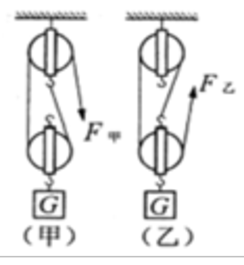
\includegraphics[width=0.5\linewidth]{图4}
\end{figure}
\columnbreak

\begin{oneparchoices}
\choice $P_\textrm{甲}>P_\textrm{乙}$ 
\choice $P_\textrm{甲}=P_\textrm{乙}$  
\choice $P_\textrm{甲}<P_\textrm{乙}$  \hspace{33pt}
\choice 无法确定
\end{oneparchoices}

\end{multicols}

\question
2013年上海市杨浦区中考物理一模试卷\\
两个完全相同的容器中,分别盛有甲、乙两种液体,将完全相同的两个小球分别放入容器中,当两球静止时,如下图所示。则物体所受的浮力为F甲、F乙;液体的密度分别为ρ甲、ρ乙它们的大小关系是(\answerline*[C])。
 \begin{multicols}{2}
\begin{figure}[H]
\centering
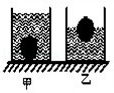
\includegraphics[width=0.5\linewidth]{图5}
\end{figure}
\columnbreak

\begin{choices}
\choice  F甲>F乙,ρ甲>ρ乙
\choice 	 F甲>F乙,ρ甲<ρ乙
\choice 	 F甲<F乙,ρ甲<ρ乙
\choice 	 F甲<F乙,ρ甲>ρ乙
\end{choices}
\end{multicols}

\end{questions}



\newpage
\section{练习题}
\begin{questions}
\question
一艘轮船在海上遭遇风暴沉没,它从开始下沉到完全没入水中前,所受到的浮力变化情况是(\answerline*[A])
\begin{choices}
\begin{multicols}{4}
\choice 增大
\choice 不变
\choice 减小
\choice 无法判断
\end{multicols}
\end{choices}


\question
小明在一支铅笔的下端粘上一块橡皮泥,将它分别置于甲、乙两杯液体中,观察到铅笔静止时的情景如下图所示,下列说法中正确的是(\answerline*[B])
\begin{multicols}{2}
\begin{choices}
\choice 甲杯液体的密度较大
\choice 乙杯液体的密度较大
\choice 铅笔在甲杯液体中受到的浮力较大
\choice 铅笔在乙杯液体中受到的浮力较大
\end{choices}
\columnbreak
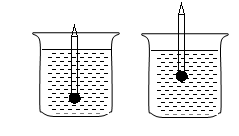
\includegraphics[scale=1]{figures/图片12.png} 
\end{multicols}


\question
一艘轮船从长江驶入东海,比较轮船在长江与东海里所受的浮力,下列说法中正确的是(\answerline*[A])
\begin{choices}
\choice 由于轮船始终浮在水面上,所以它受到的浮力不变
\choice 由于海水的密度大,所以轮船在海洋里受到的浮力大
\choice 由于轮船排开海水的体积小,所以它在海洋里受到的浮力小
\choice 由于轮船排开海水的体积大,所以它在海洋里受到的浮力大
\end{choices}


\question
装有不同液体的甲、乙两烧杯,如下图所示,放入两个完全相同的物体,当物体静止后两烧杯中液面恰好相平。液体对甲乙两烧杯底部压强分别是$P_\textrm{甲}$、$P_\textrm{乙}$,液体对两物体的浮力分别是$F_\textrm{甲}$、$F_\textrm{乙}$,下列判断正确的是(\answerline*[A])
\begin{multicols}{2}
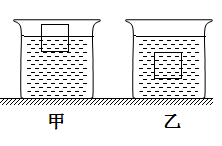
\includegraphics[scale=1]{figures/图片14.png} 
\columnbreak
\begin{choices}
\choice $P_\textrm{甲} > P_\textrm{乙}   \quad   F_\textrm{甲}=F_\textrm{乙}$ 
\choice $P_\textrm{甲} = P_\textrm{乙}   \quad   F_\textrm{甲}>F_\textrm{乙}$ 
\choice $P_\textrm{甲} = P_\textrm{乙}   \quad   F_\textrm{甲}<F_\textrm{乙}$ 
\choice $P_\textrm{甲} < P_\textrm{乙}   \quad   F_\textrm{甲}=F_\textrm{乙}$ 
\end{choices}
\end{multicols}


\question
将小铁块和小木块放入一盆水中,结果发现木块浮在水面上,铁块沉入水底,就此现象,下列分析正确的是(\answerline*[B])
\begin{choices}
\choice 木块受到浮力,铁块不受浮力
\choice 铁块沉入水底,所受浮力一定小于自身的重力
\choice 木块受到的浮力一定大于铁块所受的浮力
\choice 木块浮在水面上,所受浮力大于自身的重力
\end{choices}


\question
分别用木头、铜、铁制成甲、乙、丙三个小球,将它们放入水中,三个小球静止时位置如下图所示,以下判断正确的是(\answerline*[B])
\begin{multicols}{2}
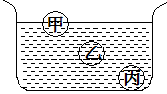
\includegraphics[scale=1]{figures/图片16.png} 
\columnbreak
\begin{choices}
\choice 甲小球一定是空心的
\choice 乙小球一定是空心的
\choice 丙小球一定是空心的
\choice 三个小球都是实心的
\end{choices}
\end{multicols}


\question
小竹将质量为$120g$的物体放入盛满水的溢水杯中,当物体静止时,溢水杯中溢出了$100cm^3$的水,则物体(\answerline*[C])($g=10N/kg$)\leftnote{水的密度$1g/cm^3$}
\begin{choices}
\choice 漂浮在水面上
\choice 悬浮在水中
\choice 沉在溢水杯底部
\choice 受到1.2N的浮力
\end{choices}


\question
关于物体所受的浮力,下列说法中正确的是(\answerline*[C])
\begin{choices}
\choice 漂浮的物体比沉底的物体受到的浮力大
\choice 物体的密度越大,受到的浮力越小
\choice 物体排开水的体积越大,受到的浮力越大
\choice 浸没在水中的物体受到的浮力与深度有关
\end{choices}           


\question
\leftnote{明确物体所受浮力就是对液体的压力}
甲、乙两个圆柱形容器盛有相同深度的液体,放置于水平桌面上,如下图所示。甲、乙两容器的底面积分别为$S_1$和$S_2$,且$2S_1=3S_2$。甲容器中液体的密度为$\rho _1$,液体对容器底产生的压强为$p_1$。乙容器中液体的密度为$\rho _2$,液体对容器底产生的压强为$p_2$,且$p_2=2p_1$。将A球浸在甲容器的液体中,B球浸在乙容器的液体中,两容器中均无液体溢出。液体静止后,甲、乙两容器底受到液体的压力相等,A、B两球所受浮力分别为$F_1$和$F_2$。则下列判断正确的是(\answerline*[A])
\begin{multicols}{2}
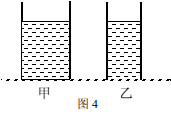
\includegraphics[scale=1]{figures/图片19.png} 
\columnbreak
\begin{choices}
\choice $F_1>F_2 \: \rho _1 < \rho _2$
\choice $F_1=F_2 \: \rho _1 < \rho _2$
\choice $F_1<F_2 \: \rho _1 > \rho _2$
\choice $F_1<F_2 \: \rho _1 < \rho _2$
\end{choices}
\end{multicols}


\question
一艘油轮满载时排水量为$5800t$,它受到的浮力为\answerline*[$5.8\times 10^7$]N,在码头卸下$8 \times 10^5kg$的燃料后,油轮排开水的体积是\answerline*[$5\times 10^3$]m。($g\textrm{取}10N/kg$)


\question
人们游泳时,会有这样的体验:当人站立在水中且身体慢慢要浸没时,池底对脚的支持力几乎为零。假如一位重$500N$的同学正在体验这种感受,则人所受浮力的大小为\answerline*[500]N,排开水的体积为\answerline*[0.05]m($g=10N/kg , \: \rho _\textrm{水}=1.0\times 10^3 kg/m^3$)
   

\question
我国自主研制的载人潜水器“蛟龙号”已“探触”$7000$米深海。当其排开海水的体积为$3m^3$时,受到浮力的大小约为\answer[60pt]{$2.94\times 10^4$}N;当其下潜至$1000$米深度时,该处海水的压强约为\answerline*[$9.8\times 10^6$]帕;该潜水器从$1000$米深处继续下潜,受到的浮力将不变(选填“变大”、“不变”或“变小”)(海水的密度近似取$1.0\times 10^3 \textrm{千克}/\textrm{米}^3$)


\end{questions}


\end{knowledge}



\begin{Aquestions}
\newpage
\section{题库A}
\begin{questions}
\question
渔民捕鱼归来,卸鱼的过程中,船受到的浮力发生变化的情况,下列说法正确的是(\answerline*[D])
\begin{choices}
\choice 浮力一定大于船受到的重力
\choice 浮力保持不变
\choice 浮力不断地增大
\choice 浮力不断地减小
\end{choices}


\question
把三个体积完全相同的球a、b、c放在水中,静止时,它们所处的位置如下图所示,下列说法中正确的是(\answerline*[C])
\begin{multicols}{2}
\begin{choices}
\choice a球受到的浮力最小
\choice b球受到的浮力最小
\choice c球受到的浮力最小
\choice 三个球受到的浮力一样大
\end{choices}
\columnbreak
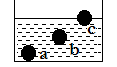
\includegraphics[scale=1]{figures/图片+14.png} 
\end{multicols}


\question
如下图所示,体积相等的三个小球静止在水中,关于它们受到的浮力大小正确是(\answerline*[D])
\begin{multicols}{2}
\begin{choices}
\choice $F_A>F_B>F_C$
\choice $F_A<F_B<F_C$
\choice $F_A >F_B=F_C$
\choice $F_A < F_B=F_C$
\end{choices}
\columnbreak
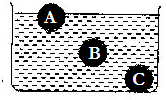
\includegraphics[scale=1]{figures/图片+15.png} 
\end{multicols}


\question
小明在课外活动中用三块大小相同的橡皮泥做成小船,把它们放在盛有水的水槽中,然后往小船内放入不同重量的物体,它们均能漂浮在水面上,如下图所示。针对此现象,下列说法正确的是(\answerline*[C])

\begin{minipage}{0.6\linewidth}
\begin{choices}
\choice 三只小船受到的浮力相等
\choice 三只小船底面受到的压力相等
\choice 小船所装物体越重,受到的浮力越大
\choice 小船所装物体越轻,受到的浮力越大
\end{choices}
\end{minipage}
\begin{minipage}{0.4\linewidth}
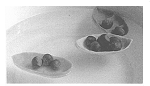
\includegraphics[scale=1]{figures/图片+16.png} 
\end{minipage}


\question
下列四个情景中,浮力增大的物体是(\answerline*[A])
\begin{choices}
\choice 从河岸沙滩走入深水处的游泳者
\choice 从长江驶入大海的轮船
\choice 海面下正在下沉的潜艇 
\choice 在码头卸载货物的货轮
\end{choices}


\question
将体积相同的实心铁球、铝球没入水中,比较它们静止时受到的浮力(已知ρ铁>ρ铝)(\answerline*[C])
\begin{choices}
\choice 铁球受到的浮力较小
\choice 铝球受到的浮力较小
\choice 铁球、铝球受到的浮力相同
\choice 在水中较深的球受到的浮力较大
\end{choices}


\question
小红在家帮妈妈洗菜,她把茄子没入水中,松手时发现茄子上浮,最后漂浮在水面上。关于茄子受到的浮力F浮与重力G的关系正确的是(\answerline*[A])
\begin{choices}
\choice 茄子上浮过程中,F浮 > G  
\choice 茄子上浮过程中,F浮 < G
\choice 茄子漂浮在水面时,F浮 > G
\choice 茄子漂浮在水面时,F浮 < G
\end{choices}


\question
在液体中流速越大的位置压强越\answerline*[小]。一艘轮船停泊在平静的海里,突然发现不远处有一危险漂浮物,为不触碰危险物,使用消防水管喷水(不便于直接喷危险物)使它近离轮船,在下图所示中水管应沿着\answerline*[P1P2]喷水 (选填“O1O2”或“P1P2”)

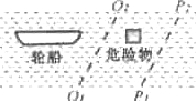
\includegraphics[scale=1]{figures/图片+20.jpg} 


\question
把一小球放入盛满酒精(密度为$0.8\times 10^3 kg/m^3$)深度为$20cm$的溢水杯中,它沉入容器底部,从杯中溢出$8g$酒精,杯底受到酒精的压强为\answerline*[$1.6\times 10^3$]Pa;若将该小球放入盛满水的溢水杯中,它漂浮在水面上,从杯中溢出水的质量\answerline*[大于]$8g$(选填“大于”、“小于”或“等于”)。(取$g=10N/kg$。)


\question
如下图所示,潜水艇能够上浮和下沉是通过改变\answer[70pt]{自身的重力}来实现的;潜水艇在上浮过程中,未露出水面之前,所受的浮力将\answerline*[不变](选填“变大”、“变小”或“不变”)。

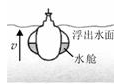
\includegraphics[scale=1]{figures/图片+22.png} 


\question
如下图所示,盛热水的茶杯中有一片茶叶,茶叶上附有两个球形气泡,此时它恰好处于悬浮状态,茶叶与两个气泡的总体积为$1\times 10^{-8}m^3$,则这片茶叶的重力为\answerline*[$
1\times 10^{-4}$]N。若在茶杯上盖紧盖子,会发现这片茶叶将\answerline*[下沉](选填“上浮”、“下沉”或“悬浮”)。($g=10N/kg$)

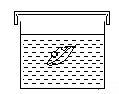
\includegraphics[scale=1]{figures/图片+23.png} 


\question
刚倒入玻璃杯中的雪碧会产生很多小气泡。此时,将一些葡萄干加入杯中,有些葡萄干会沉入杯底,这些葡萄干表面因吸附足够的小气泡,受到的浮力\answerline*[大于]重力,从而上浮;上浮到液面后,由于小气泡破裂,导致它们受到的浮力\answerline*[小于]重力,于是又沉入杯底(选填“大于”或“小于”)。


\question
在某次抗洪救灾中,武警某部官兵利用冲锋舟为人民群众开辟了水上生命线,该冲锋舟自重为$0.6\times 10^4$N,满载时排开水的体积为$1.5m^3$,吃水深度为$0.5m$。(已知$\rho _\textrm{水} = 1.0\times 10^3kg/m^3$,取$g=10N/kg$),求:
\begin{enumerate}
\item 冲锋舟满载时底部所受水的压强多大?
\item 冲锋舟满载时所受的浮力是多少?
\item 假设每人的平均质量为60kg,为保证安全,冲锋舟最多能承载多少人?
\end{enumerate}

\begin{solution}[26ex]
1.冲锋舟底部$0.5m$深处所受水的压强为:
\[p=\rho _\textrm{水} g h =1.0\times 10^3 kg/m^3 \times 10N/kg \times 0.5m = 5 \times 10^3 Pa\]

2.冲锋舟满载时所受的浮力为:
\[F_\textrm{浮}=\rho _\textrm{水} g V_ \textrm{排} = 1.0\times 10^3 kg/m^3  \times 10N/kg \times 1.5m^3=1.5 \times 10^4 N \]

3.冲锋舟满载时,设人的总重为$G_\textrm{人}$,有$G_\textrm{舟}+G_\textrm{人}=F_\textrm{浮}$即$0.6 \times 10^4 +G_\textrm{人}  =1.5 \times 10 ^4 N$ \\
求得:$G_\textrm{人}=0.9\times 10^4 N$\\
由题意可知:$G_\textrm{每人}=mg=60kg\times 10 N/kg=600N$\\
所以冲锋舟最多承载的人数为:$n=\frac{G_\textrm{人}}{G_\textrm{每人}}=15(\textrm{人})$
\end{solution}


\end{questions}
\end{Aquestions}



%\section{小信息}
%\showendnotes

\ThisCenterWallPaper{1}{教案模板-3.pdf}

\end{document}



